\documentclass[tikz]{standalone}
\usepackage{ctex}
\usepackage{tikz}
\usepackage{pgfplots}
\pgfplotsset{compat=1.18}   % 使用较新版本语法
\usetikzlibrary{positioning, arrows.meta, intersections, calc, fit, backgrounds}
\usepgfplotslibrary{fillbetween}  % 用于填充区域
\begin{document}
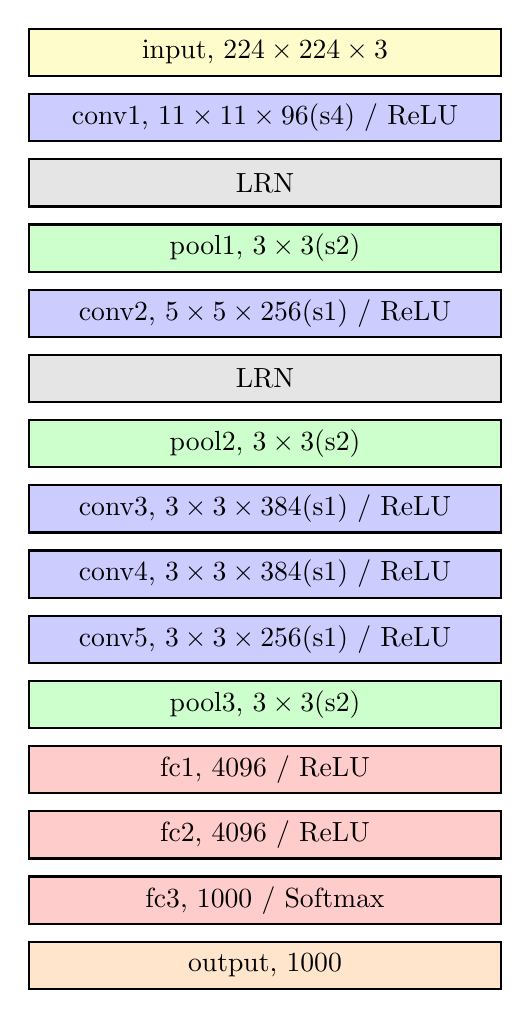
\begin{tikzpicture}[
    ->,>=stealth,shorten >=1pt,auto,thick,
    node distance = 0.2cm,
    >=Stealth,
    conv/.style={draw, minimum width=6cm, minimum height=0.6cm, fill=blue!20},
    pool/.style={draw, minimum width=6cm, minimum height=0.6cm, fill=green!20},
    fc/.style={draw, minimum width=6cm, minimum height=0.6cm, fill=red!20},
    input/.style={draw, minimum width=6cm, minimum height=0.6cm, fill=yellow!20},
    output/.style={draw, minimum width=6cm, minimum height=0.6cm, fill=orange!20},
    activate/.style={draw, minimum width=6cm, minimum height=0.6cm, fill=purple!20},
    norm/.style={draw, minimum width=6cm, minimum height=0.6cm, fill=gray!20},
]

\node[input] (input) {input, $224\times 224\times 3$};
\node[conv, below=of input] (conv1) {conv1, $11 \times 11 \times 96$(s4) / ReLU};
\node[norm, below=of conv1] (lrn1) {LRN};
\node[pool, below=of lrn1] (pool1) {pool1, $3 \times 3$(s2)};
\node[conv, below=of pool1] (conv2) {conv2, $5 \times 5 \times 256$(s1) / ReLU};
\node[norm, below=of conv2] (lrn2) {LRN};
\node[pool, below=of lrn2] (pool2) {pool2, $3 \times 3$(s2)};
\node[conv, below=of pool2] (conv3) {conv3, $3 \times 3 \times 384$(s1) / ReLU};
\node[conv, below=of conv3] (conv4) {conv4, $3 \times 3 \times 384$(s1) / ReLU};
\node[conv, below=of conv4] (conv5) {conv5, $3 \times 3 \times 256$(s1) / ReLU};
\node[pool, below=of conv5] (pool3) {pool3, $3 \times 3$(s2)};
\node[fc, below=of pool3] (fc1) {fc1, 4096 / ReLU};
\node[fc, below=of fc1] (fc2) {fc2, 4096 / ReLU};
\node[fc, below=of fc2] (fc3) {fc3, 1000 / Softmax};
\node[output, below=of fc3] (output) {output, 1000};
\end{tikzpicture}
\end{document}